\section{Dimension One: A Geometric Look at the Real Line}

Although we assume the reader is familiar with the real numbers $\mathbb{R}$, it is beneficial to revisit them from a more grown-up geometric perspective to set the stage for higher dimensions. The real line is a set $\mathbb{R}$ of elements that are conventionally called numbers. However in geometry, their names and their role depends on the context. For example, when we visualize $\mathbb{R}$ as a line in space, each element corresponds to a specific location. In this context, we refer to elements of $\mathbb{R}$ as \textbf{points}.

\subsection{Translations and Vectors}

Elements of $\mathbb{R}$ have another geometric interpretation: they can represent \textbf{translations} or shifts (in this book we use the two words interchangeably). For example, the number $v \in \mathbb{R}$ can associated with the operation of shifting the origin (or any other point) by $v$ units to the right.

Formally, for any fixed number $v \in \mathbb{R}$, we can define a translation operator $T_v: \mathbb{R} \to \mathbb{R}$ by:
\[ T_v(x) = x + v \]
This operator takes a point $x$ and shifts it by $v$, obtaining the point $x+v$. When we think of elements of $\mathbb{R}$ as defining these shift operators, it is often helpful to visualize them as \textbf{arrows} rather than points, which visually correspond to the shift operation.

An arrow can be drawn starting at the origin $0$ and ending at $v$ to represent the shift $v$. However, the same shift operation can be applied to any point. Thus, we can draw an arrow starting at any point $x$ and ending at $x+v$ to represent the same shift $v$.
Formally, we can think of an arrow as a pair of points $(x, y)$, where $x$ is the \emph{tail} (or anchor) and $y$ is the \emph{head}. This arrow represents the displacement from $x$ to $y$.

\begin{figure}[h]
    \centering
    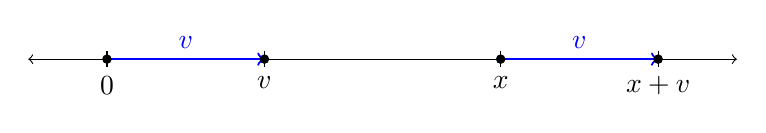
\begin{tikzpicture}
        % Number line
        \draw[<->] (-1,0) -- (8,0);
        \foreach \x in {0,2,5,7} \draw (\x,0.1) -- (\x,-0.1);
        \node[below] at (0,-0.1) {$0$};
        \node[below] at (2,-0.1) {$v$};
        \node[below] at (5,-0.1) {$x$};
        \node[below] at (7,-0.1) {$x+v$};
        
        % Vector v from origin
        \draw[->, thick, blue] (0,0) -- (2,0) node[midway, above] {$v$};
        
        % Vector v from x
        \draw[->, thick, blue] (5,0) -- (7,0) node[midway, above] {$v$};
        
        % Points
        \filldraw (0,0) circle (1.5pt);
        \filldraw (2,0) circle (1.5pt);
        \filldraw (5,0) circle (1.5pt);
        \filldraw (7,0) circle (1.5pt);
    \end{tikzpicture}
    \caption{Visualizing a vector $v$ as a translation. The blue arrows represent the same vector $v$, acting as a displacement from $0$ to $v$ and from $x$ to $x+v$. Both arrows represent the same geometric object.}
    \label{fig:vector_translation}
\end{figure}

Two arrows $(x, y)$ and $(x', y')$ are considered \textbf{equivalent} if they represent the same displacement, which means:
\[ y - x = y' - x' \]
(in which case one can define $z=y-x$, and the arrows become $(x, x+z)$ and $(x', x'+z)$ respectively)
This indeed defines an equivalence relation on the set of all arrows. An equivalence class thus contains arrows which correspond to the same displacement. Thus while each arrow in an equivalence class is a different object, they all signify the same geometric concept. We thus define a \textbf{vector} to be an equivalence class of arrows under this relation.
This vector captures the abstract notion of "magnitude and direction" (in 1D, direction is just sign) of a shift, which can be respresented by an arrow but are independent of its starting point. Note that for a vector $v$ which contains the arros $(x,y)$, $v$ is uniquely identified by the number $y-x$. We therefore sometimes say, somewhat abusing definitions, "the vector $z$" when we actually mean the equivalence class of arrows $\set{(x, x+z)}_{x\in\mathbb{R}}$. 

\subsection{Geometric Objects}

The concept of defining a geometric object as an equivalence class extends beyond vectors.
Consider a shape, like an interval $[a, b] \subset \mathbb{R}$. If we shift this interval by some amount $v$, we get a new set $[a+v, b+v]$. Intuitively, these two sets represent the "same" geometric shape, just in different locations.

We can define a \textbf{shape} as an equivalence class of subsets of $\mathbb{R}$ under translation. Two sets $A, B \subset \mathbb{R}$ determine the same shape if there exists a translation $v$ such that:
\[ B = \{ a + v \mid a \in A \} \]

\begin{figure}[h]
    \centering
    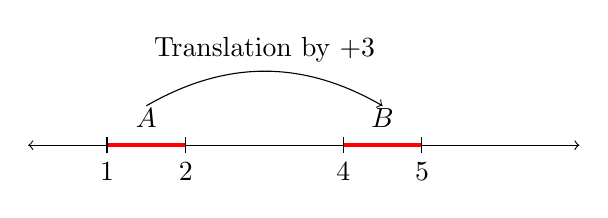
\begin{tikzpicture}
        % Number line
        \draw[<->] (0,0) -- (7,0);
        
        % Interval A [1,2]
        \draw[ultra thick, red] (1,0) -- (2,0);
        \node[above] at (1.5,0.1) {$A$};
        \draw (1,0.1) -- (1,-0.1);
        \draw (2,0.1) -- (2,-0.1);
        \node[below] at (1,-0.1) {$1$};
        \node[below] at (2,-0.1) {$2$};
        
        % Interval B [4,5] (translated by 3)
        \draw[ultra thick, red] (4,0) -- (5,0);
        \node[above] at (4.5,0.1) {$B$};
        \draw (4,0.1) -- (4,-0.1);
        \draw (5,0.1) -- (5,-0.1);
        \node[below] at (4,-0.1) {$4$};
        \node[below] at (5,-0.1) {$5$};

        % Translation arrow
        \draw[->, bend left] (1.5,0.5) to node[above] {Translation by $+3$} (4.5,0.5);
    \end{tikzpicture}
    \caption{The sets $A=[1,2]$ and $B=[4,5]$ represent the same geometric shape because one is a translation of the other.}
    \label{fig:shape_equivalence}
\end{figure}

We can generalize this even further. Consider a pair of subsets, or more generally, a tuple of subsets of $\mathbb{R}$. We can naturally translate the entire tuple by applying translation to each component.
We define a \textbf{geometric object} as an equivalence class of tuples of subsets of $\mathbb{R}$ under translation (for simplicity, we allow single point in a tuple so that we can avoid singletons).
For instance, consider an arrow consisting of a pair of points $(x, y)$. If we shift both $x$ and $y$ by the same $z$, we get an equivalent arrow $(x+z, y+z)$ -- this captures the relative position of the sets within the tuple.
Vectors are thus a special case of geometric objects where the tuple consists of two single point.  This broad definition of geometric objects allows us to study properties that depend on the configuration of multiple shapes relative to each other, and are invariant under the absolute position in space.

A \textbf{geometric property} can be viewed in two equivalent ways. First, it is a property of tuples of sets which is invariant under translations. For example, the property "the distance between the two points is 5" is a geometric property of a pair of points $(x, y)$, because shifting the pair does not change their distance. Equivalently, it is a property of geometric objects, namely of equivalence classes of tuples of subsets of $\mathbb{R}$ under translation. Since all tuples in an equivalence class share the same invariant properties, we can ascribe the property to the class as a whole. Thus, "length" is a property of the vector (or interval) itself, independent of where it is located in space.

\begin{figure}[h]
    \centering
    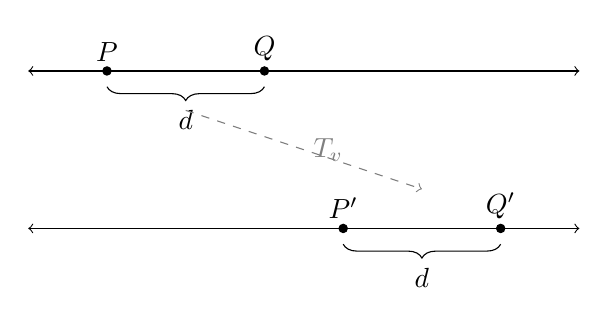
\begin{tikzpicture}
        % Configuration 1
        \draw[<->] (-1,2) -- (6,2);
        \filldraw (0,2) circle (1.5pt) node[above] {$P$};
        \filldraw (2,2) circle (1.5pt) node[above] {$Q$};
        \draw[decorate,decoration={brace,amplitude=5pt,mirror}] (0,1.8) -- (2,1.8) node[midway,below=5pt] {$d$};
        
        % Configuration 2
        \draw[<->] (-1,0) -- (6,0);
        \filldraw (3,0) circle (1.5pt) node[above] {$P'$};
        \filldraw (5,0) circle (1.5pt) node[above] {$Q'$};
        \draw[decorate,decoration={brace,amplitude=5pt,mirror}] (3,-0.2) -- (5,-0.2) node[midway,below=5pt] {$d$};
        
        % Translation arrow
        \draw[->, dashed, gray] (1,1.5) -- (4,0.5) node[midway, right] {$T_v$};
    \end{tikzpicture}
    \caption{Geometric properties, such as the distance $d$ between two points, are invariant under translation.}
    \label{fig:geometric_invariance}
\end{figure}

